\documentclass[hyperref={pdfpagelabels=false}]{beamer}
\usepackage{beamerthemesplit}
\usepackage[utf8]{inputenc}
\usepackage[T1]{fontenc}
\usepackage{lmodern}
\usepackage[french]{babel}
\usepackage{graphicx}
\usepackage{tikz}

\uselanguage{French}
\languagepath{French}
\usetheme{Green}

\begin{document}
\title{Le logiciel de preuves formelles Coq}
\author{Guillaume Claret}
\date{12 mars 2015}
\maketitle

\section{Démo}
% All template changes are local to this group.
{
  \setbeamertemplate{navigation symbols}{}
  \begin{frame}[plain]
    \frametitle{Démo}
    \begin{tikzpicture}[remember picture,overlay]
      \node[at=(current page.center)] {
        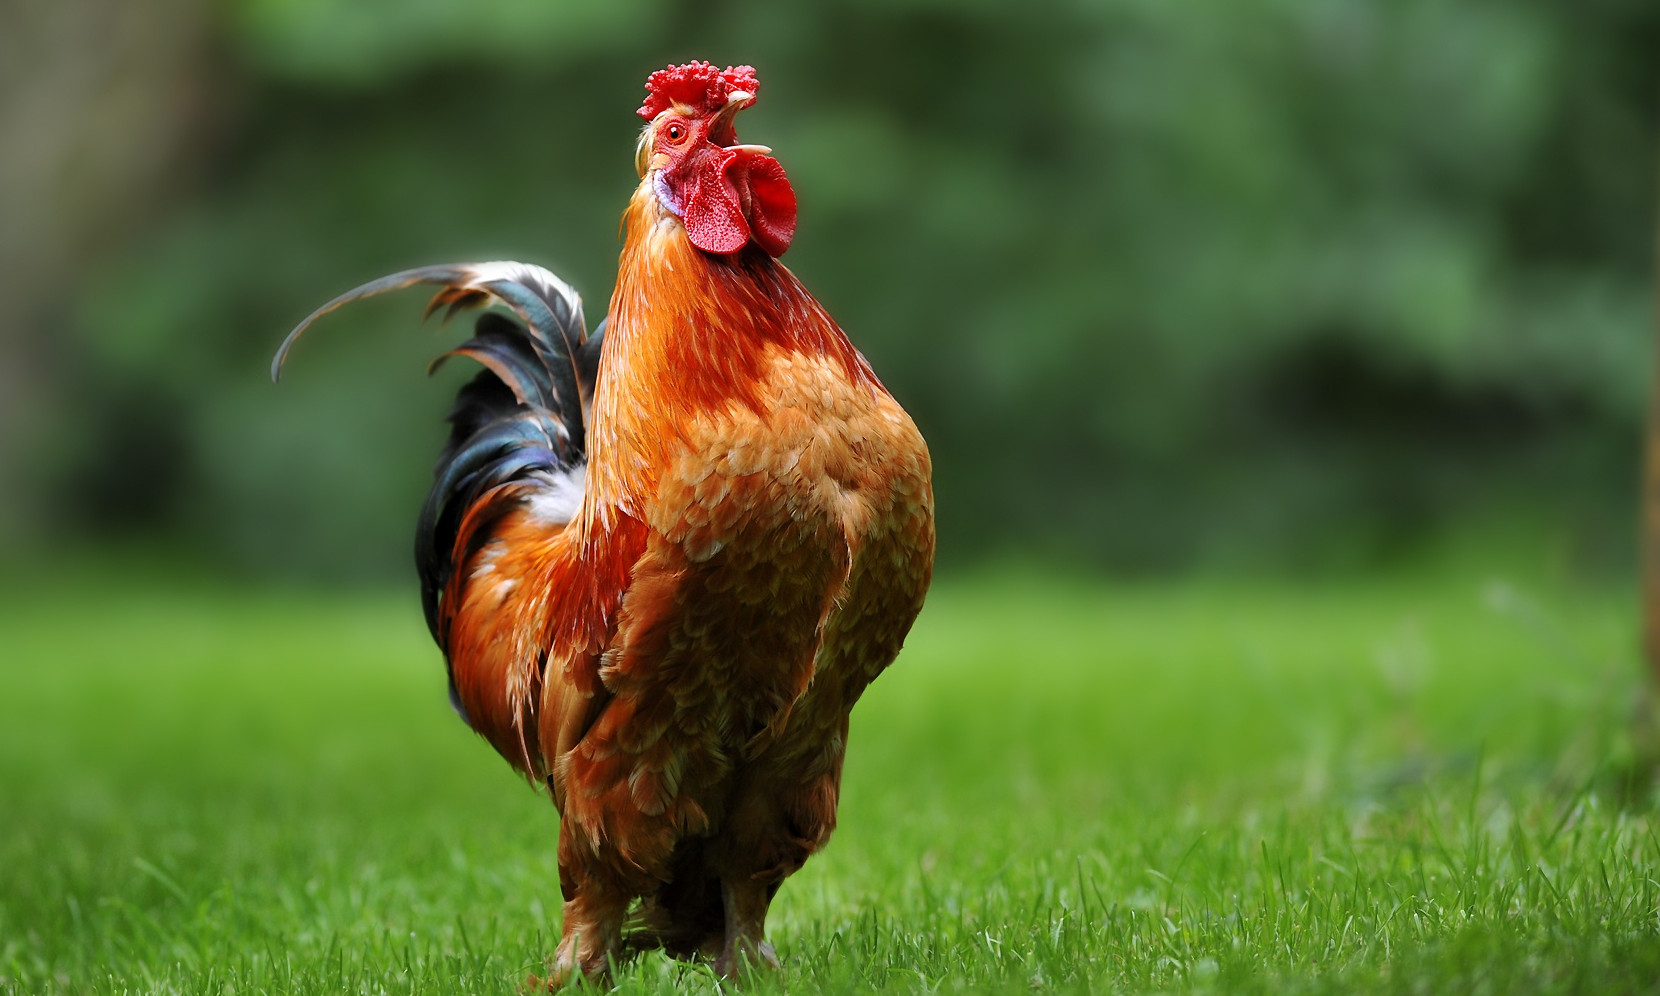
\includegraphics[width=\paperwidth]{images/coq}
      };
    \end{tikzpicture}
  \end{frame}
}

\section{Présentation}
\begin{frame}
  \frametitle{Le logiciel Coq}
  Un language pour:
  \begin{itemize}
    \item énoncer des théorèmes
    \item écrire des preuves formelles
    \item écrire des algorithmes
  \end{itemize}

  Un environnement pour:
  \begin{itemize}
    \item raisonner de façon interactive
    \item organiser / distribuer les développements
  \end{itemize}
\end{frame}

\begin{frame}
  \frametitle{Développements importants}
  \begin{itemize}
    \item théorème des quatre couleurs (Gontier 04)
    \item théorème de Feit -- Thompson (Gontier \& all, 12)
    \item compilateur \textsc{C} CompCert (Xavier Leroy \& all)
    \item bibliothèque \emph{Bedrock} de vérification de programmes bas niveau
  \end{itemize}
\end{frame}

\begin{frame}
  \frametitle{Historique}
  \begin{itemize}
    \item Calcul des Constructions (\textsc{CoC}) par \emph{Thierry Coquand} (85)
    \item implémentation du \textsc{CoC} donnant lieu à \textsc{Coq}
    \item Calculus of Inductive Constructions (\textsc{CiC}) par \emph{Christine Paulin} (91)
  \end{itemize}
\end{frame}
\end{document}
